\documentclass[tikz,border=3mm]{standalone}
\usepackage{pgfplots}
\pgfplotsset{compat=1.16}

\usepgfplotslibrary{patchplots}
\begin{document}
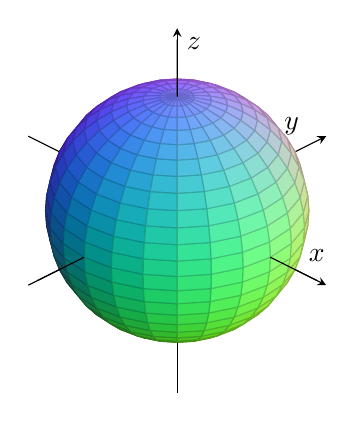
\begin{tikzpicture}
\begin{axis}[axis equal,
        width=10cm,
        height=10cm,
        axis lines = center,
        xlabel = {$x$},
        ylabel = {$y$},
        zlabel = {$z$},
        ticks=none,
        enlargelimits=0.3,
        z buffer=sort,
        view/h=45,
        scale uniformly strategy=units only]
% this example burns colors if opacity 
% is active in the document.
    \addplot3 [patch,
        patch type=bilinear,
        mesh/color input=explicit mathparse,
        variable = \u,
        variable y = \v,
        domain = 0:360,
        y domain = 0:180,
        point meta={symbolic={0.5+0.5*y, % R
        0.5+0.5*x, % G 
            0.5+0.5*z%B
            } },
    ] ({cos(u)*sin(v)}, {sin(u)*sin(v)}, {cos(v)});
  \draw (1,0,0) -- (1.5,0,0) (0,-1,0)   -- (0,-1.5,0) (0,0,1)   -- (0,0,1.5);
\end{axis}
\end{tikzpicture}
\end{document}
